\documentclass[12pt]{article}
\usepackage[english]{babel}
\usepackage{natbib}
\usepackage{url}
\usepackage[utf8x]{inputenc}
\usepackage{amsmath}
\usepackage{graphicx}
\usepackage{hyperref}
\graphicspath{{images/}}
\usepackage{parskip}
\usepackage{fancyhdr}
\usepackage{vmargin}
\setmarginsrb{3 cm}{2.5 cm}{3 cm}{2.5 cm}{1 cm}{1.5 cm}{1 cm}{1.5 cm}

\title{Sentiment Analysis on Movie Reviews}								% Title
\author{(Chaitanay S.,Pranjal G., Sagar J.)}								% Author
\date{\today}											% Date

\makeatletter
\let\thetitle\@title
\let\theauthor\@author
\let\thedate\@date
\makeatother

\pagestyle{fancy}
\fancyhf{}
\rhead{\theauthor}
\lhead{\thetitle}
\cfoot{\thepage}

\begin{document}

%%%%%%%%%%%%%%%%%%%%%%%%%%%%%%%%%%%%%%%%%%%%%%%%%%%%%%%%%%%%%%%%%%%%%%%%%%%%%%%%%%%%%%%%%

\begin{titlepage}
	\centering
    \vspace*{0.5 cm}
    
\includegraphics[scale = 0.75]{logo.jpg}\\[1.0 cm]	% University Logo
    \textsc{\LARGE IIIT BANGALORE}\\[2.0 cm]	% University Name			
	\textsc{\large Course Name - Machine Learning}\\[0.5 cm]				% Course Name
	\rule{\linewidth}{0.2 mm} \\[0.4 cm]
	{ \huge \bfseries \thetitle}\\
	\rule{\linewidth}{0.2 mm} \\[1.5 cm]
	
	\begin{minipage}{0.4\textwidth}
		\begin{flushleft} \large
			\emph{Author:}\\
			\theauthor
			\end{flushleft}
			\end{minipage}~
			\begin{minipage}{\textwidth}
			\begin{flushright} \large
			\emph \noindent {Roll Num:} \\
			MT2018027,\newline MT2018081,\newline MT2018097 \newline
												% Your Student Number
		\end{flushright}
	\end{minipage}\\[2 cm]
	
	{\large \thedate}\\[2 cm]
 
	\vfill
	
\end{titlepage}

%%%%%%%%%%%%%%%%%%%%%%%%%%%%%%%%%%%%%%%%%%%%%%%%%%%%%%%%%%%%%%%%%%%%%%%%%%%%%%%%%%%%%%%%%

\tableofcontents
\pagebreak

%%%%%%%%%%%%%%%%%%%%%%%%%%%%%%%%%%%%%%%%%%%%%%%%%%%%%%%%%%%%%%%%%%%%%%%%%%%%%%%%%%%%%%%%%





\maketitle
\thispagestyle{empty}
\pagestyle{empty}


%%%%%%%%%%%%%%%%%%%%%%%%%%%%%%%%%%%%%%%%%%%%%%%%%%%%%%%%%%%%%%%%%%%%%%%%%%%%%%%%
\begin{abstract}

This document is the project report for Sentiment Analysis on movie reviews- Based on the reviews given by the user we need to predict the sentiment behind the statement made.

\end{abstract}


%%%%%%%%%%%%%%%%%%%%%%%%%%%%%%%%%%%%%%%%%%%%%%%%%%%%%%%%%%%%%%%%%%%%%%%%%%%%%%%%
\section{INTRODUCTION}

In this project- Sentiment Analysis on Movie Reviews, the dataset given to us consisted of the fields- Phraseid, Sentenceid, Phrase, Sentiment. By processing the phrase given using any relevant model we had to predict the sentiment of the user.

\section{FEATURE ENGINEERING}

\subsection{INTRODUCTION}

Feature engineering is the process of using domain knowledge of the data to create features that make machine learning algorithms work. 
\newline
    In the dataset given to us, the phrase consisted of textual data which can
not be an input to the machine learning algorithm and hence the basic idea of Feature Engineering was to convert the textual data to some numeric values do that we can make the Machine Learning Algorithms work.    

\subsection{NEW FEATURES INCLUDED}

\begin{itemize}
    \item A feature called 'total length' was added, which had the total number of letters in the phrase.

\item A new feature called 'words' was added, it contains the total number of words in the phrase.
\item Another feature which kept track of the average length of a words in the phrase was also added.
\item Another feature which kept track of number of paragraphs was also added.
\item Another feature which kept track of number of stop words was also added. Stop words refer to the most common words in a language.
\item Another feature which kept track of exclamation marks and the average number of excalamtion marks in the phrase was added to the dataset.
\item Another feature that kept the average number of question marks was added.
\item Another feature which kept track of the number of unique words in the phrase also added.
\item Feature which kept track of repeated words in a phrase was added.
\item Features which kept track of number of nouns,number of adjectives and number of verbs was also added.
\end{itemize}

\section{Exploratory Data Analysis (EDA)}

\begin{itemize}
    \item A plot b/w number of phrases in each sentiment was plotted and it showed that the given data is unbalanced as huge of amount of phrases were categorized as neutral.
    
    \begin{figure}[h!]
  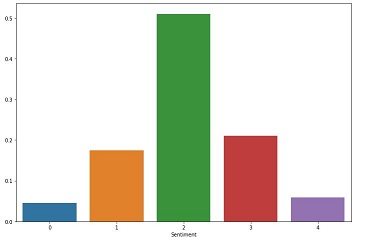
\includegraphics[width=\linewidth]{EDA1.JPG}
  \caption{ Number of phrases of a particular Sentiment}
  \label{fig:Graph1}
\end{figure}


 \item A Correlation matrix was plotted b/w the features and the target label and then it showed that number of words and no of stop words, unique words showed more correlation than other features.This gave an idea to use the tfidf and count vectors as features. 
 
  \begin{figure}[h!]
  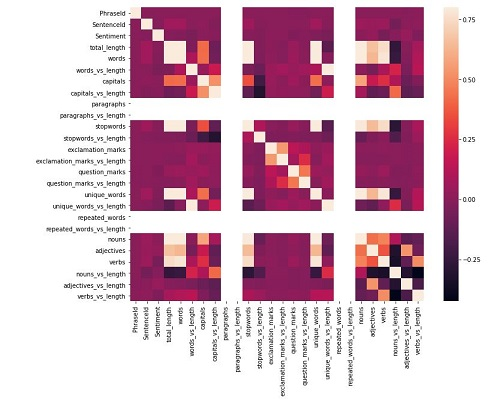
\includegraphics[width=\linewidth]{jj.JPG}
  \caption{ Correlation Matrix between the features and the target label}
  \label{fig:Graph1}
\end{figure}

\item Tf-idf stands for term frequency-inverse document frequency, and the tf-idf weight is a weight often used in information retrieval and text mining. This weight is a statistical measure used to evaluate how important a word is to a document in a collection or corpus. The importance increases proportionally to the number of times a word appears in the document but is offset by the frequency of the word in the corpus. Variations of the tf-idf weighting scheme are often used by search engines as a central tool in scoring and ranking a document's relevance given a user query.




    \item TF: Term Frequency, which measures how frequently a term occurs in a document. Since every document is different in length, it is possible that a term would appear much more times in long documents than shorter ones. Thus, the term frequency is often divided by the document length (aka. the total number of terms in the document) as a way of normalization:

    \item TF(t) = (Number of times term t appears in a document) / (Total number of terms in the document).

    \item IDF: Inverse Document Frequency, which measures how important a term is. While computing TF, all terms are considered equally important. However it is known that certain terms, such as "is", "of", and "that", may appear a lot of times but have little importance. Thus we need to weigh down the frequent terms while scale up the rare ones, by computing the following:

    \item IDF(t) = log\textsubscript{e}(Total number of documents / Number of documents with term t in it).
    \end{itemize}

\section{Data Preprocessing}

\subsection{Introduction}
\begin{itemize}
    \item The dataset provided was very unclean. The punctuations were not at the right place and there were some single word and single letter phrases which did not convey any sentiment. This conclusion was based on the visualization of the dataset.
    \end{itemize}
    
\subsection{What has been done ?}
\begin{itemize}
    \item To avoid any undesired discrepancies in the data all the words were converted to lowercase alphabets.
    \item The stop words i.e. the common words in a language were removed from the dataset since they are common words and do not help in conveying any sentiment. e.g. is, an, the etc.
    \item The rare words i.e. the words that have occured only one to two times in the dataset were removed from the dataset.
\end{itemize}

\subsection{Stemming}
\begin{itemize}
    \item Stemming is the process of reducing inflected (or sometimes derived) words to their word stem, base or root form—generally a written word form.
    \item Example: studies --> studi, studying --> study etc.
    
\end{itemize}

\subsection{Lemmatization}
\begin{itemize}
    \item Lemmatization on the other hand ,takes in to consideration analysis of the words. To do so, it is necessary to have detailed dictionaries which the algorithm can look through to link the form back to its lemma.
    \item Example: studies -> study, studying -> study etc.
    \item Lemmatization was preferred in this project because of it being more effective in catching the semantics of the word and reducing the redundancy of the similar type of words.

\subsection{Vectorizer used}
 \begin{itemize}
     \item Tfidf was used initially to imply the importance of a word in the given phrase.It gave a relatively low score as compared to the upcoming trials.
     \item Count Vectorizer was used to specify the frequency of a particular word in the dataset. This resulted in a better score as compared to the Tfidf implementation.
     \item The dataset was tested by using a stacked version of the Tfidf and the count Vectorizer. This gave the best result as compared to using count vectorizer or Tfidf independently and hence this technique has been employed in the prediction.The parameters used as an input to the count vectorizer were: input='content',
    encoding='utf-8',decode\_error='strict',
    strip\_accents=None,lowercase=True,preprocessor=None,
    tokenizer=None,
    stop\_words=None,
    token\_pattern=r"(?u)\b\w\w+\b",ngram\_range=(1,2),
    analyzer='word',
    max\_df=1.0,
    min\_df=1,max\_features=None,
    vocabulary=None,binary=False,
    dtype=np.float64.
 \end{itemize}

\subsubsection{CountVector and TF-IDF Vector}
\begin{itemize}
    \item CountVectors and TF-IDF vectors were stacked together on the pre-processed data to act as an input for the algorithms. TF-IDF conveying the importance of each word and countvector simply the number of counts of words.
\end{itemize}
\end{itemize}
 \section{MODEL BUILDING}
 A number of models were built and tested on different set of input features.They all gave different results due to different reasons, this section explains why the set of features were given and why the results were the way there were.
 \subsection{Logistic Regression}
 \begin{itemize}
     \item The features that were included by the process of Feature Engineering were used as the input vector and then Logistic Regression was used in order to test the accuracy of the data which resulted in a 0.62 score. This was obvious as the correlation matrix showed that there was not a great correlation between the extracted features and the targeted sentiment.
     
 \end{itemize}
 
 
 
 \subsection{XG Boost}
 \begin{itemize}
     \item XG Boost was employed by using the output vector from the Tfidf vectorizer as an input to the XG Boost Classifier. This model resulted in an accuracy of 0.65. The Parameters used for applying this model were:  booster='gbtree',colsample\_bylevel=1,
       colsample\_bytree=1,gamma=0,max\_delta\_step=0,
       max\_depth=8,min\_child\_weight=1,
       missing=None,n\_jobs=1,
       nthread=4,objective='multi:softmax',num\_class=5,
       random\_state=0,
       reg\_alpha=0,
       reg\_lambda=1,scale\_pos\_weight=1,seed=None,
       silent=True,
       subsample=1.
 \end{itemize}
 
 \subsection{Naive Bayes}
 \begin{itemize}
     \item Naive Bayes was used in order to increase the accuracy for the targeted sentiment but the best score that it was able to pull off was 0.63.
 \end{itemize}
 
 \subsection{Ensemble}
 \begin{itemize}
     \item We tried stacking up the Logistic Regression model, XG boost along with Naive Bayes in order to improve the aaccuracy that was observed by applying these models alone. This Ensemble resulted in an accuracy of 0.71 in public leaderboard and 0.
 \end{itemize}
\subsection{Logistic Regression-2}
\begin{itemize}
    \item  A logistic regression model was trained on the stack of tfidf vectors and count vectors, this resulted in the highest accuracy this project was able to achieve, the Test Data in the public leaderboard resulted in 0.73 score while the test data in the private leaderboard resulted in a 0.67 score. The parameters used for applying this model were: dual=False, tol=0.0001,fit\_intercept=True,
    intercept\_scaling=1, 
    class\_weight=None,random\_state=None,C=1.0,
    max\_iter=100,
    solver='newton-cg',
    multi\_class='multinomial',verbose=0,warm\_start=False,
    n\_jobs=None
\end{itemize}

\section{Picke File Link}

\subsection {Link}
\begin{itemize}
    \item \url{https://iiitborg-my.sharepoint.com/:f:/g/personal/sagar_jhunjhunwala_iiitb_org/EmwxyDYcfndMseZJ-J3MyhgBdKfWvNqczms_9fgKgRySBg?e=EdU0xO}
\end{itemize}



\section{CONCLUSION}

The data was very impure and hence we did the best possible data preprocessing and feature engineering we could think of. We tried including new features during the feature engineering process and tried to get some correlation between the features and the targeted sentiment. We tried applying lots of models but the model that resulted in the best accuracy was Logistic Regression along with Count Vectorizer that gave an accuracy of 0.73 on public leaderboard and 0.67 on private leaderboard.

\addtolength{\textheight}{-12cm}   % This command serves to balance the column lengths
                                  % on the last page of the document manually. It shortens
                                  % the textheight of the last page by a suitable amount.
                                  % This command does not take effect until the next page
                                  % so it should come on the page before the last. Make
                                  % sure that you do not shorten the textheight too much.

%%%%%%%%%%%%%%%%%%%%%%%%%%%%%%%%%%%%%%%%%%%%%%%%%%%%%%%%%%%%%%%%%%%%%%%%%%%%%%%%



%%%%%%%%%%%%%%%%%%%%%%%%%%%%%%%%%%%%%%%%%%%%%%%%%%%%%%%%%%%%%%%%%%%%%%%%%%%%%%%%



%%%%%%%%%%%%%%%%%%%%%%%%%%%%%%%%%%%%%%%%%%%%%%%%%%%%%%%%%%%%%%%%%%%%%%%%%%%%%%%%

\section*{ACKNOWLEDGMENT}

We would like to thank Sir GSR Raghavan along with all the TA's for helping us and guiding us all through the process. This was a great learning curve for all of us and we have definetely learnt a lot from this project.



%%%%%%%%%%%%%%%%%%%%%%%%%%%%%%%%%%%%%%%%%%%%%%%%%%%%%%%%%%%%%%%%%%%%%%%%%%%%%%%%



\begin{thebibliography}{99}

\bibitem{c1} Kaggle - We have referred to several kernels that pre-existed on Kaggle that helped us to kick-start the project.

\bibitem{c2} Documentations - We have taken reference from several documentations of libraries that were used in the project.

\end{thebibliography}
\end{document}